\subsection{Problem 1}

In a simple linear regression with one covariate $X_i$:

\subsection*{(a)}

Show that the estimates for the slope and intercept are
\[
\widehat{\beta} = \frac{\sum_{i=1}^{n}(X_i - \overline{X}_n)(Y_i - \overline{Y}_n)}{\sum_{i=1}^{n}(X_i - \overline{X}_n)^2}
\]
and
\[
\widehat{\alpha} = \overline{Y}_n - \widehat{\beta}\overline{X}_n.
\]

Hint:
\[
\begin{pmatrix} a & b \\ b & c \end{pmatrix}^{-1} = \frac{1}{ac - b^2} \begin{pmatrix} c & -b \\ -b & a \end{pmatrix}
\]

\textbf{Solution.}

设简单线性回归模型为 $Y_i = \beta X_i + \alpha + \varepsilon_i$，拟合值为 $\widehat{Y} = \widehat{\beta} X + \widehat{\alpha}$。

最小二乘法的目标是最小化残差平方和：
\[
\sum_{i=1}^{n}(Y_i - \alpha - \beta X_i)^2
\]

对 $\alpha$ 求偏导并令其为0：
\[
\frac{\partial}{\partial \alpha} = -2\sum_{i=1}^{n}(Y_i - \alpha - \beta X_i) = 0
\]
\[
\Rightarrow \sum_{i=1}^{n} Y_i - n\alpha - \beta\sum_{i=1}^{n} X_i = 0
\]
\[
\Rightarrow \widehat{\alpha} = \overline{Y} - \beta\overline{X}
\]

对 $\beta$ 求偏导并令其为0：
\[
\frac{\partial}{\partial \beta} = -2\sum_{i=1}^{n} X_i(Y_i - \alpha - \beta X_i) = 0
\]
\[
\Rightarrow \sum_{i=1}^{n} X_i Y_i - \alpha\sum_{i=1}^{n} X_i - \beta\sum_{i=1}^{n} X_i^2 = 0
\]

将上述两个方程写成矩阵形式：
\[
\begin{pmatrix} n & \sum X_i \\ \sum X_i & \sum X_i^2 \end{pmatrix} \begin{pmatrix} \alpha \\ \beta \end{pmatrix} = \begin{pmatrix} \sum Y_i \\ \sum X_i Y_i \end{pmatrix}
\]

解得：
\[
\begin{pmatrix} \widehat{\alpha} \\ \widehat{\beta} \end{pmatrix} = \frac{1}{n\sum X_i^2 - (\sum X_i)^2} \begin{pmatrix} \sum X_i^2 & -\sum X_i \\ -\sum X_i & n \end{pmatrix} \begin{pmatrix} \sum Y_i \\ \sum X_i Y_i \end{pmatrix}
\]

因此：
\[
\widehat{\beta} = \frac{-\sum X_i \sum Y_i + n\sum X_i Y_i}{n\sum X_i^2 - (\sum X_i)^2}
\]

整理（同除以 $n$）：
\[
\widehat{\beta} = \frac{\sum_{i=1}^{n}(X_i - \overline{X})(Y_i - \overline{Y})}{\sum_{i=1}^{n}(X_i - \overline{X})^2}
\]

\hfill $\blacksquare$

\subsection*{(b)}

Show that $R^2$ is the squared Pearson's correlation between $Y_i$'s and $X_i$'s.

\textbf{Solution.}

已知：
\[
R^2 = \frac{\sum(\widehat{Y}_i - \overline{Y})^2}{\sum(Y_i - \overline{Y})^2}, \quad \text{Cor}(X,Y) = \frac{[\sum(X_i - \overline{X})(Y_i - \overline{Y})]^2}{\sum(X_i - \overline{X})^2 \sum(Y_i - \overline{Y})^2}
\]

由 $\widehat{Y}_i = \widehat{\alpha} + \widehat{\beta} X_i$，可得：
\[
\sum(\widehat{Y}_i - \overline{Y})^2 = \sum[\widehat{\alpha} + \widehat{\beta} X_i - \widehat{\alpha} - \widehat{\beta}\overline{X}]^2 = \widehat{\beta}^2 \sum(X_i - \overline{X})^2
\]

又因为：
\[
\sum(X_i - \overline{X})(Y_i - \overline{Y}) = \sum(X_i - \overline{X})(\widehat{\alpha} + \widehat{\beta} X_i - \widehat{\alpha} - \widehat{\beta}\overline{X}) = \widehat{\beta}\sum(X_i - \overline{X})^2
\]

代入上式，则：
\[
R^2 = \widehat{\beta}^2 \frac{\sum(X_i - \overline{X})^2}{\sum(Y_i - \overline{Y})^2}
\]

因此：
\[
\text{Cor}(X,Y) = \frac{\widehat{\beta}^2 [\sum(X_i - \overline{X})^2]^2}{\sum(X_i - \overline{X})^2 \sum(Y_i - \overline{Y})^2} = \widehat{\beta}^2 \frac{\sum(X_i - \overline{X})^2}{\sum(Y_i - \overline{Y})^2} = R^2
\]

\hfill $\blacksquare$

\newpage

\subsection{Problem 2}

(Framingham study) Consider the \textbf{log-transformed cholesterol level} as the outcome.

\subsection*{(a)}

Fit a \textbf{linear model} of the outcome on one covariate, \textbf{BMI}.

\subsubsection*{(i)}

Test the null hypothesis of no BMI effect. Visualize the data to check their relationship.

\textbf{Solution.}

符号同problem 1，结果如下：
\[
\widehat{\alpha} = 5.37, \quad \widehat{\beta} = 0.00364
\]

$p\text{-value} < 2 \times 10^{-16}$，拒绝原假设。

\begin{center}
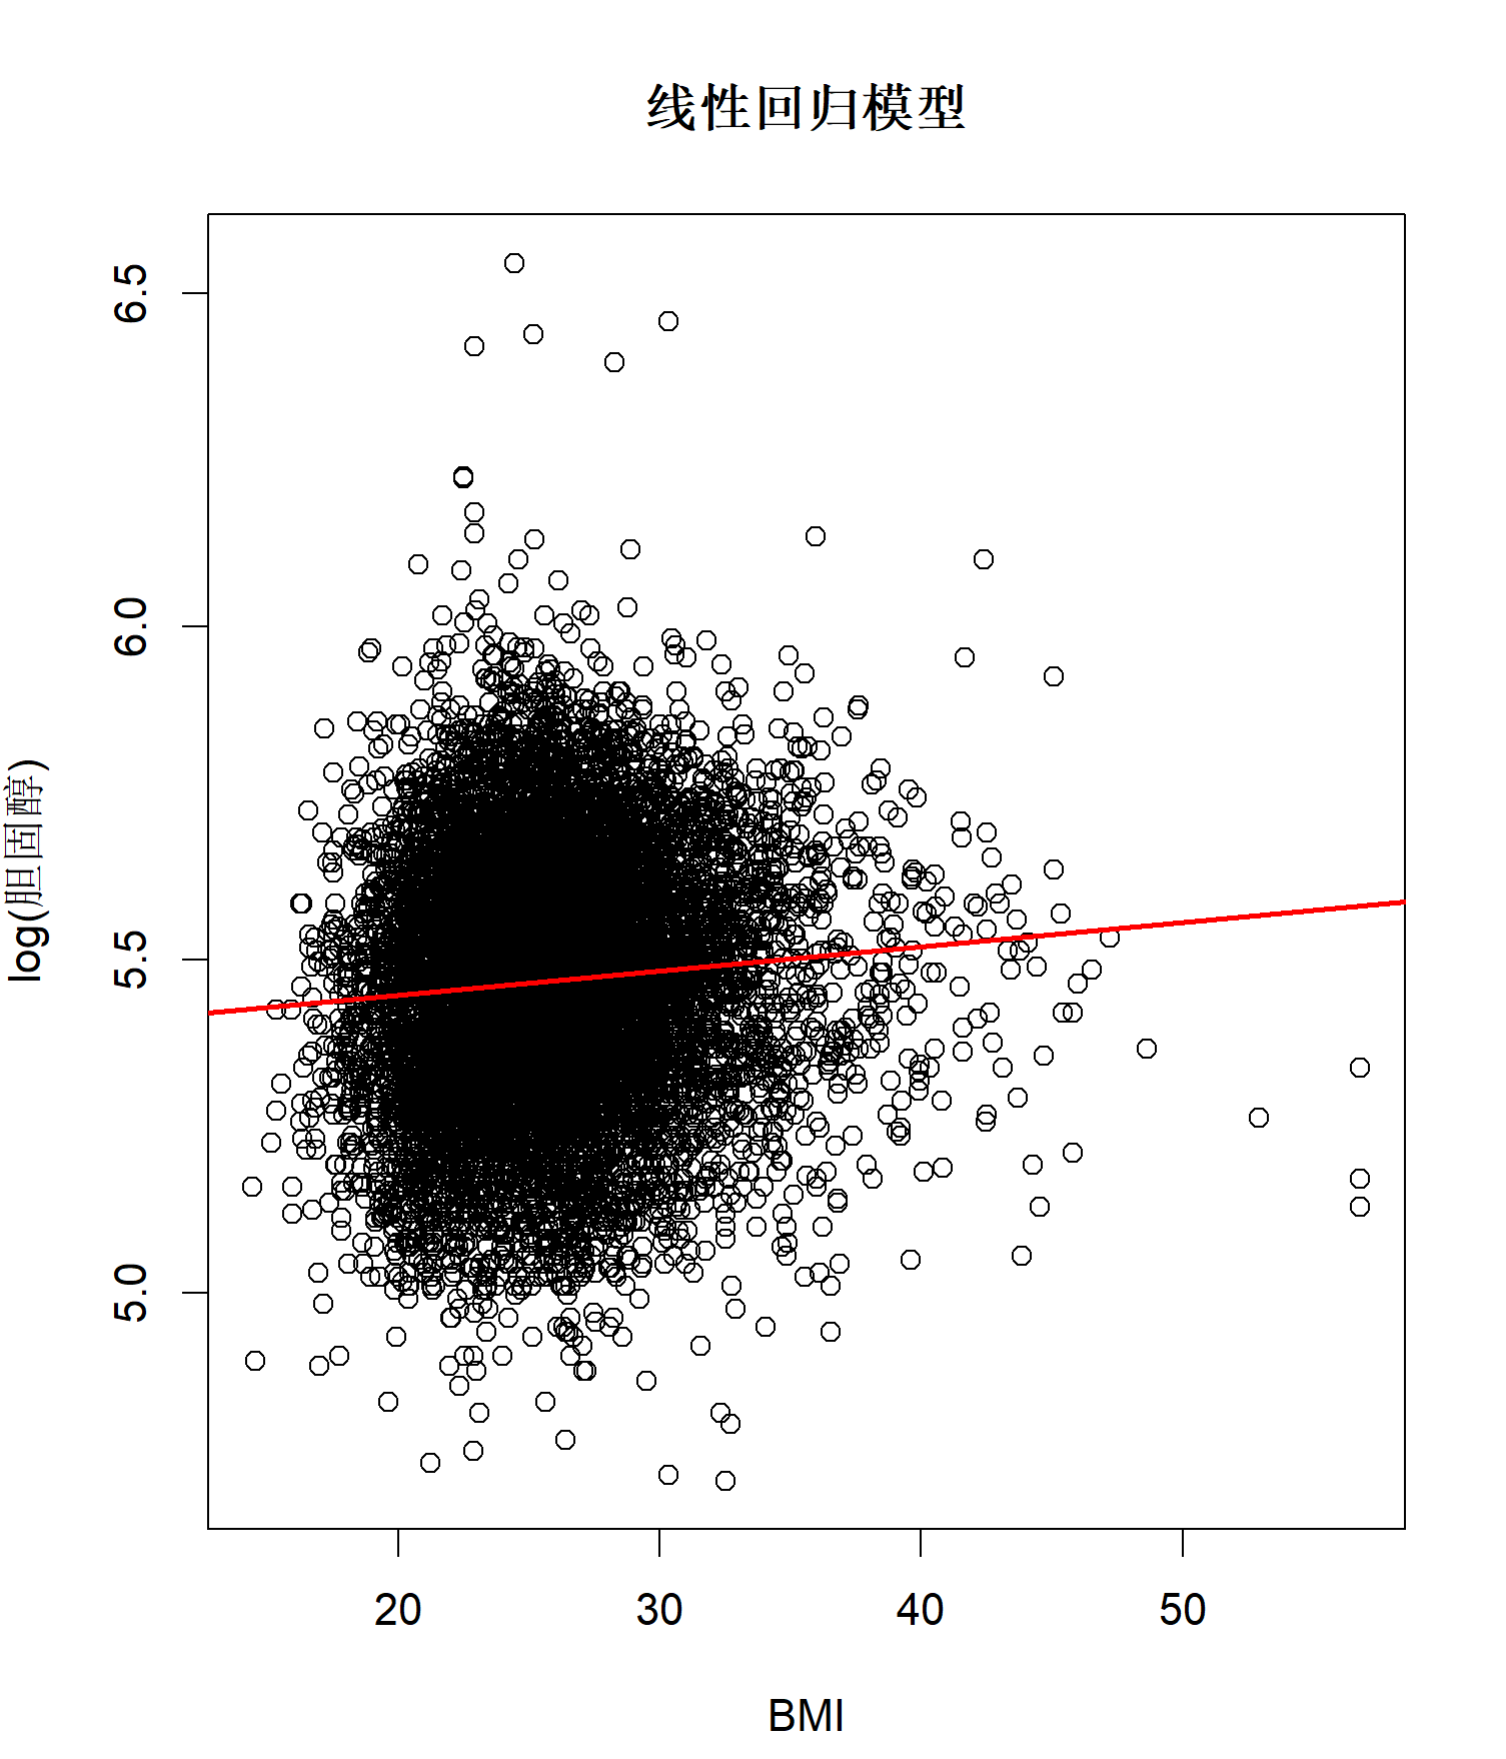
\includegraphics[width=0.7\textwidth]{figs/hw4_bmi_logcholesterol_scatter.png}
\end{center}

图中可以看出二者正相关。

\subsubsection*{(ii)}

Report the $R^2$ value and verify that it is the squared Pearson correlation when there is only one predictor.

\textbf{Solution.}

$R^2 = 0.006311$

$\rho^2 = 0.006311$，本问在problem 1的基础上用数据验证了 $R^2 = \rho^2$。

remark：数据点很多，虽然这里 $R^2$ 十分小但是仍然可以有显著相关性。

\subsubsection*{(iii)}

Plot the residuals to check:
\begin{itemize}
    \item whether the linear model is correctly specified,
    \item whether the errors are normal and homogeneous,
    \item whether there is any outlier.
\end{itemize}

\textbf{Solution.}

\begin{center}
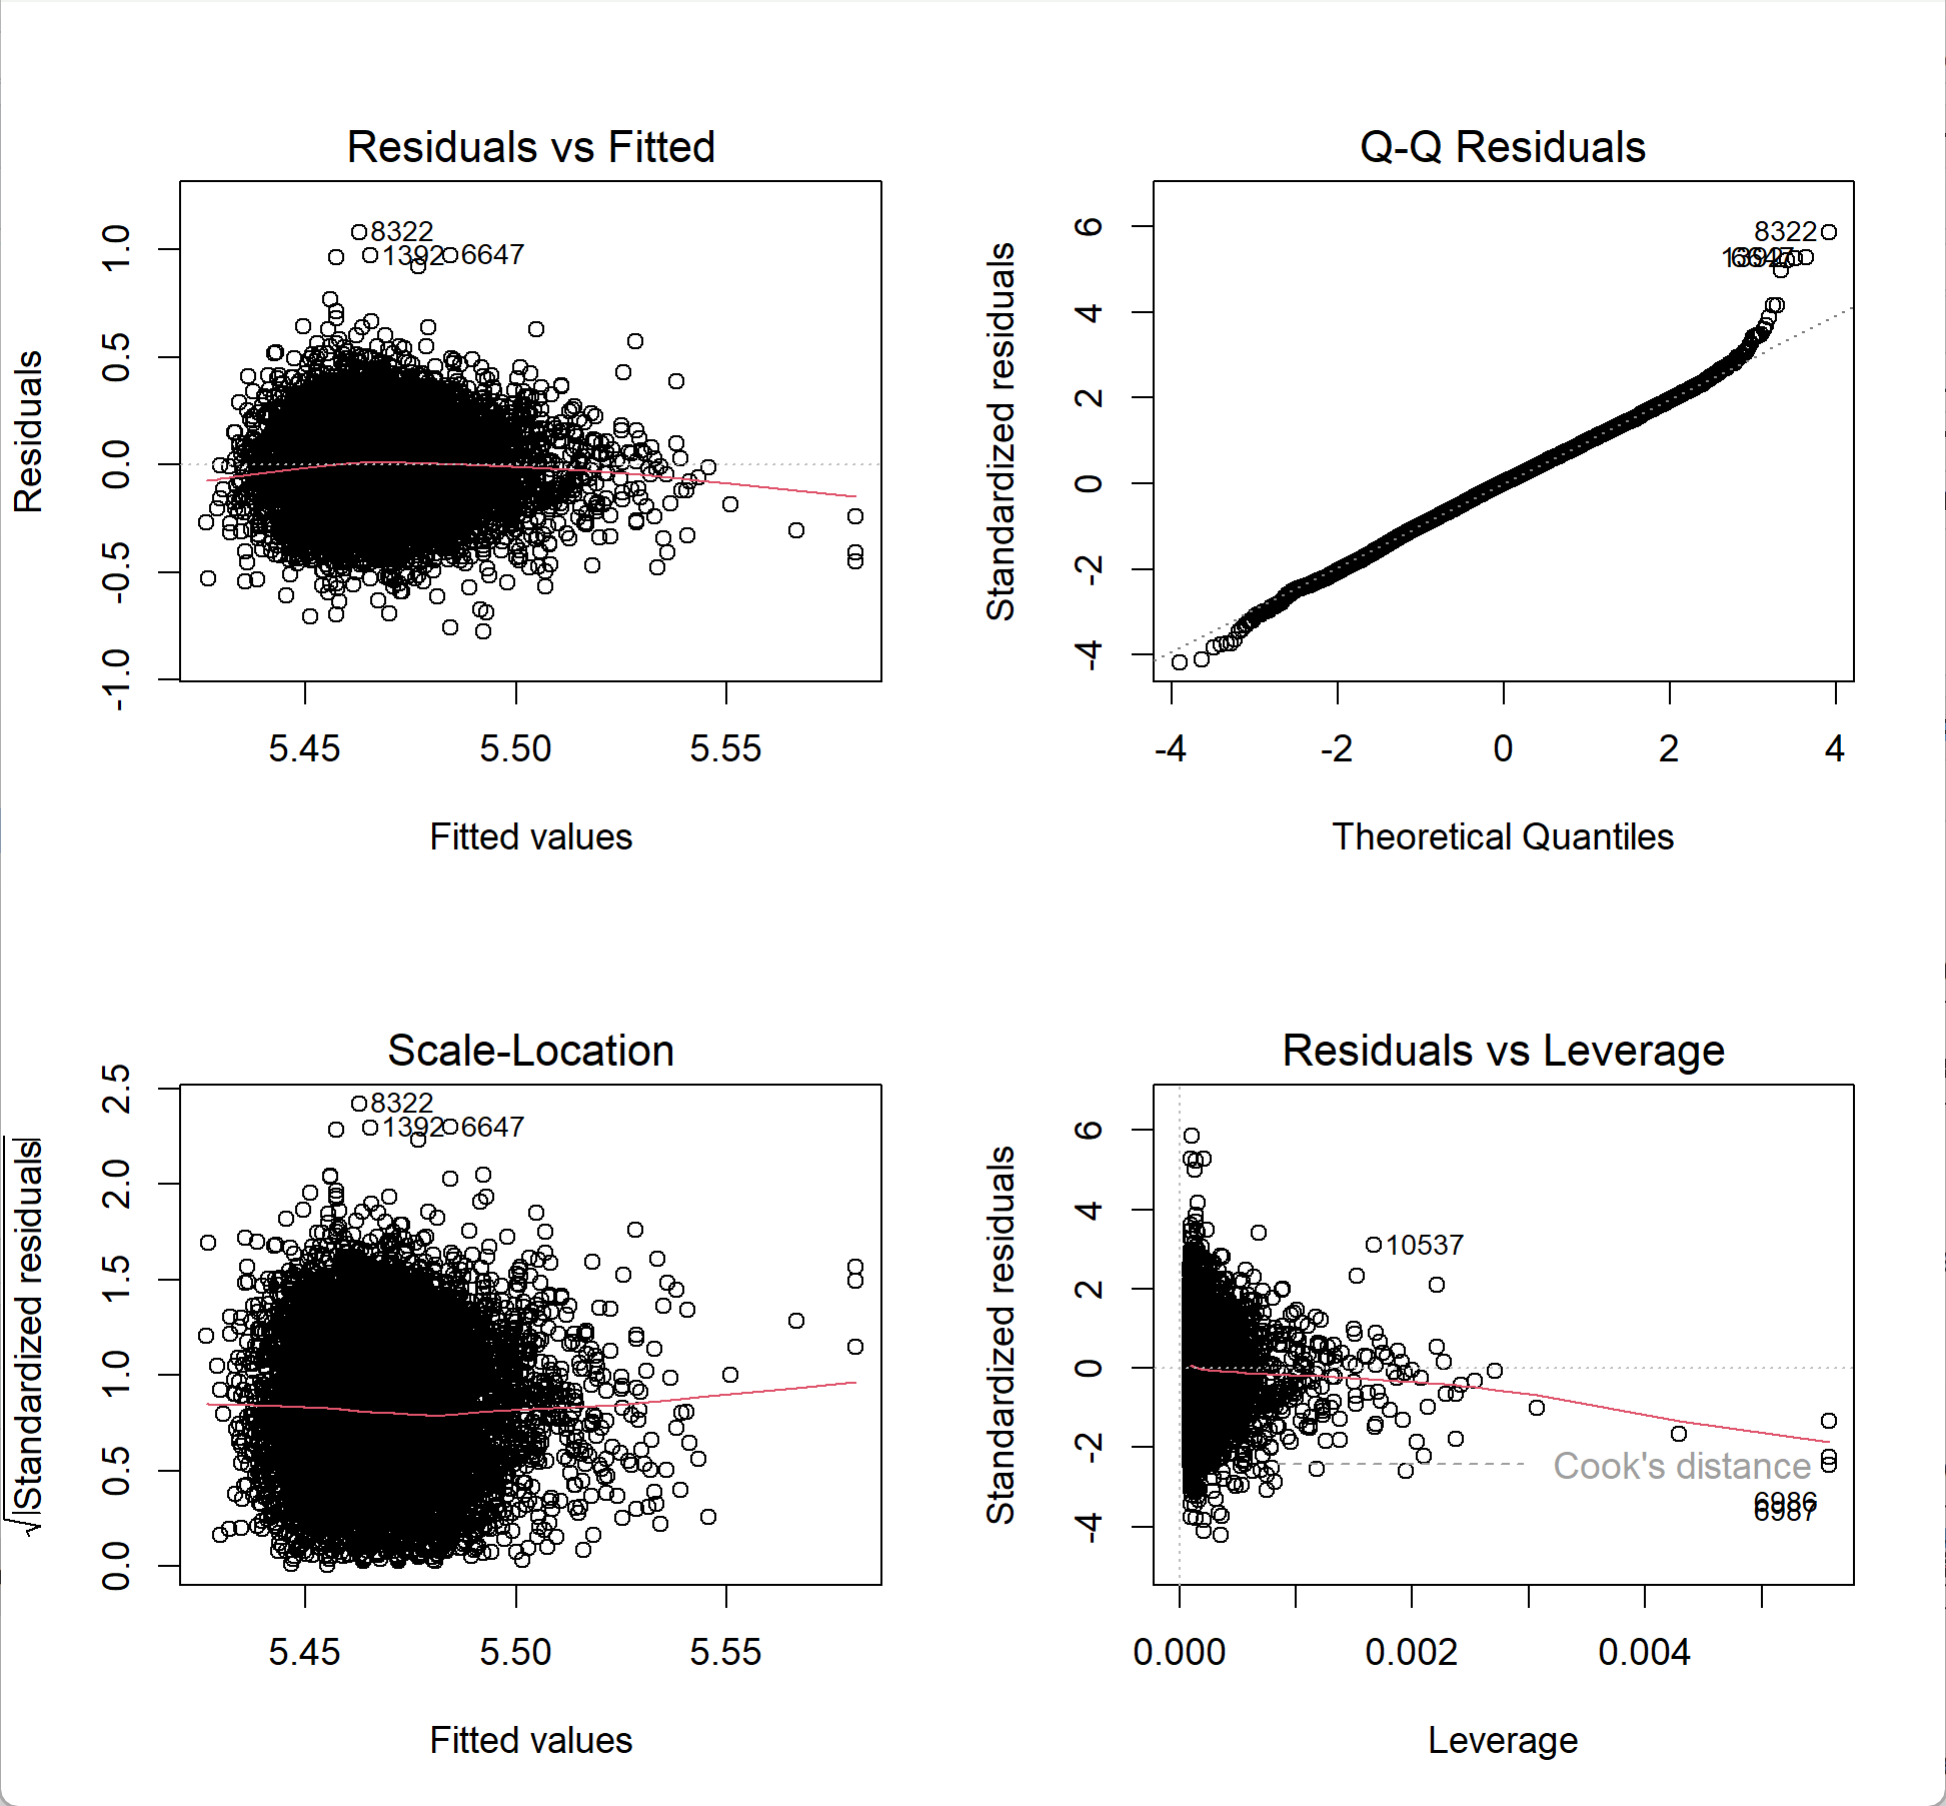
\includegraphics[width=0.8\textwidth]{figs/hw4_bmi_residuals.png}
\end{center}

\begin{itemize}
    \item 基本正确，Residuals vs Fitted 图中残差拟合线虽然有一定弧度但均接近0；残差在0两侧分布基本均匀。scale-location 图拟合线基本水平，没有出现明显的异方差情况。说明对线性模型的假设基本正确。
    \item 根据Q-Q Residuals 图，误差基本服从正态分布，但右尾有一定偏移，说明数据虽然经过对数变换但仍然存在重尾现象。
    \item 有极少的离群值，已在图中标注。
\end{itemize}

综上，使用线性模型是合理的。

\subsection*{(b)}

Fit an \textbf{ANOVA} model of the outcome on \textbf{age group}.

\subsubsection*{(i)}

Test the null hypothesis of no age effect. Visualize the data to check their relationship.

\textbf{Solution.}

\begin{center}
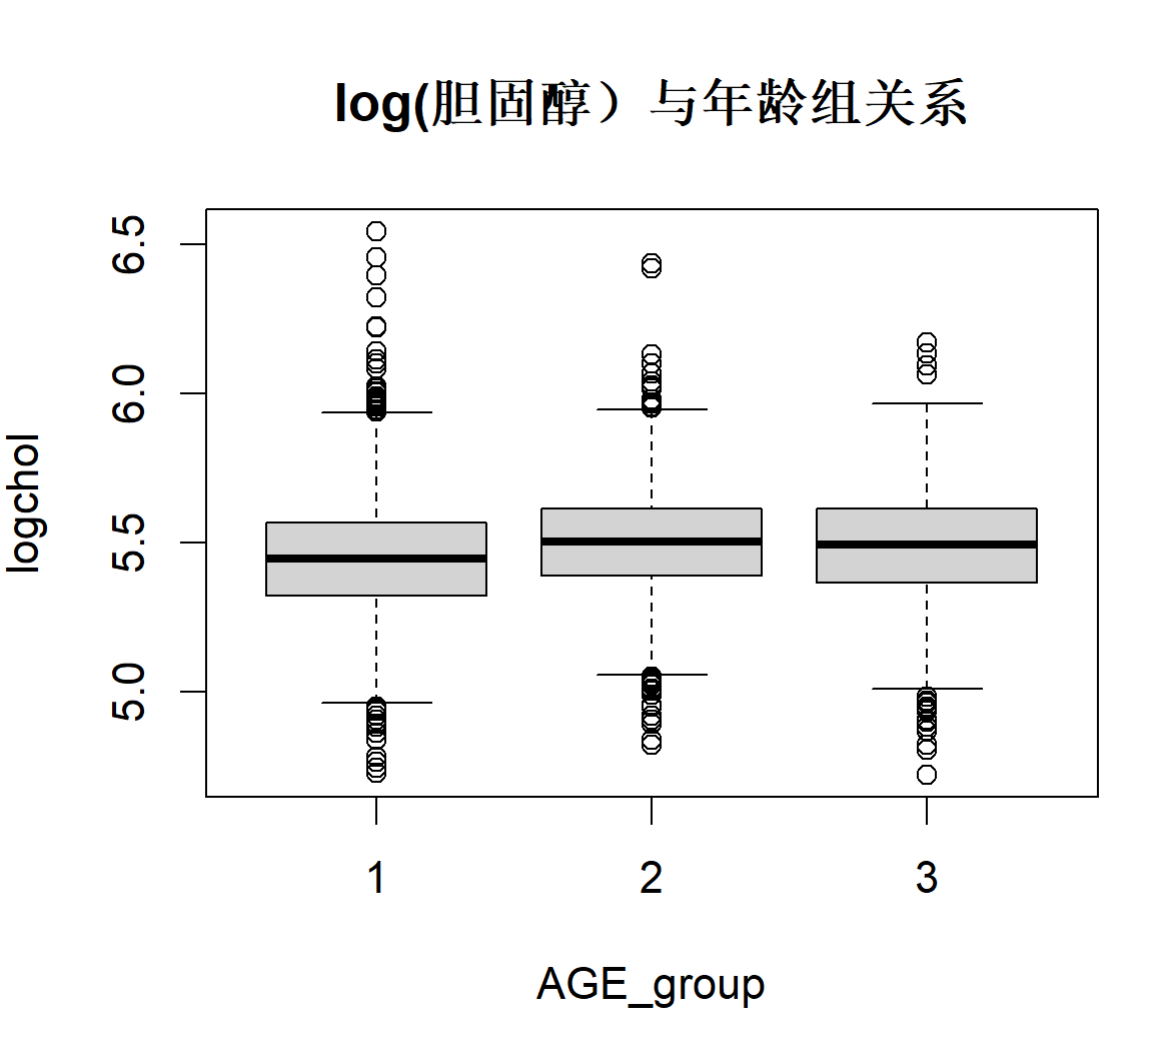
\includegraphics[width=0.7\textwidth]{figs/hw4_age_boxplot.png}
\end{center}

$p\text{-value} < 2 \times 10^{-16}$，拒绝原假设。

\subsubsection*{(ii)}

Plot the residuals to assess the normality and homogeneity of errors.

\textbf{Solution.}

\begin{center}
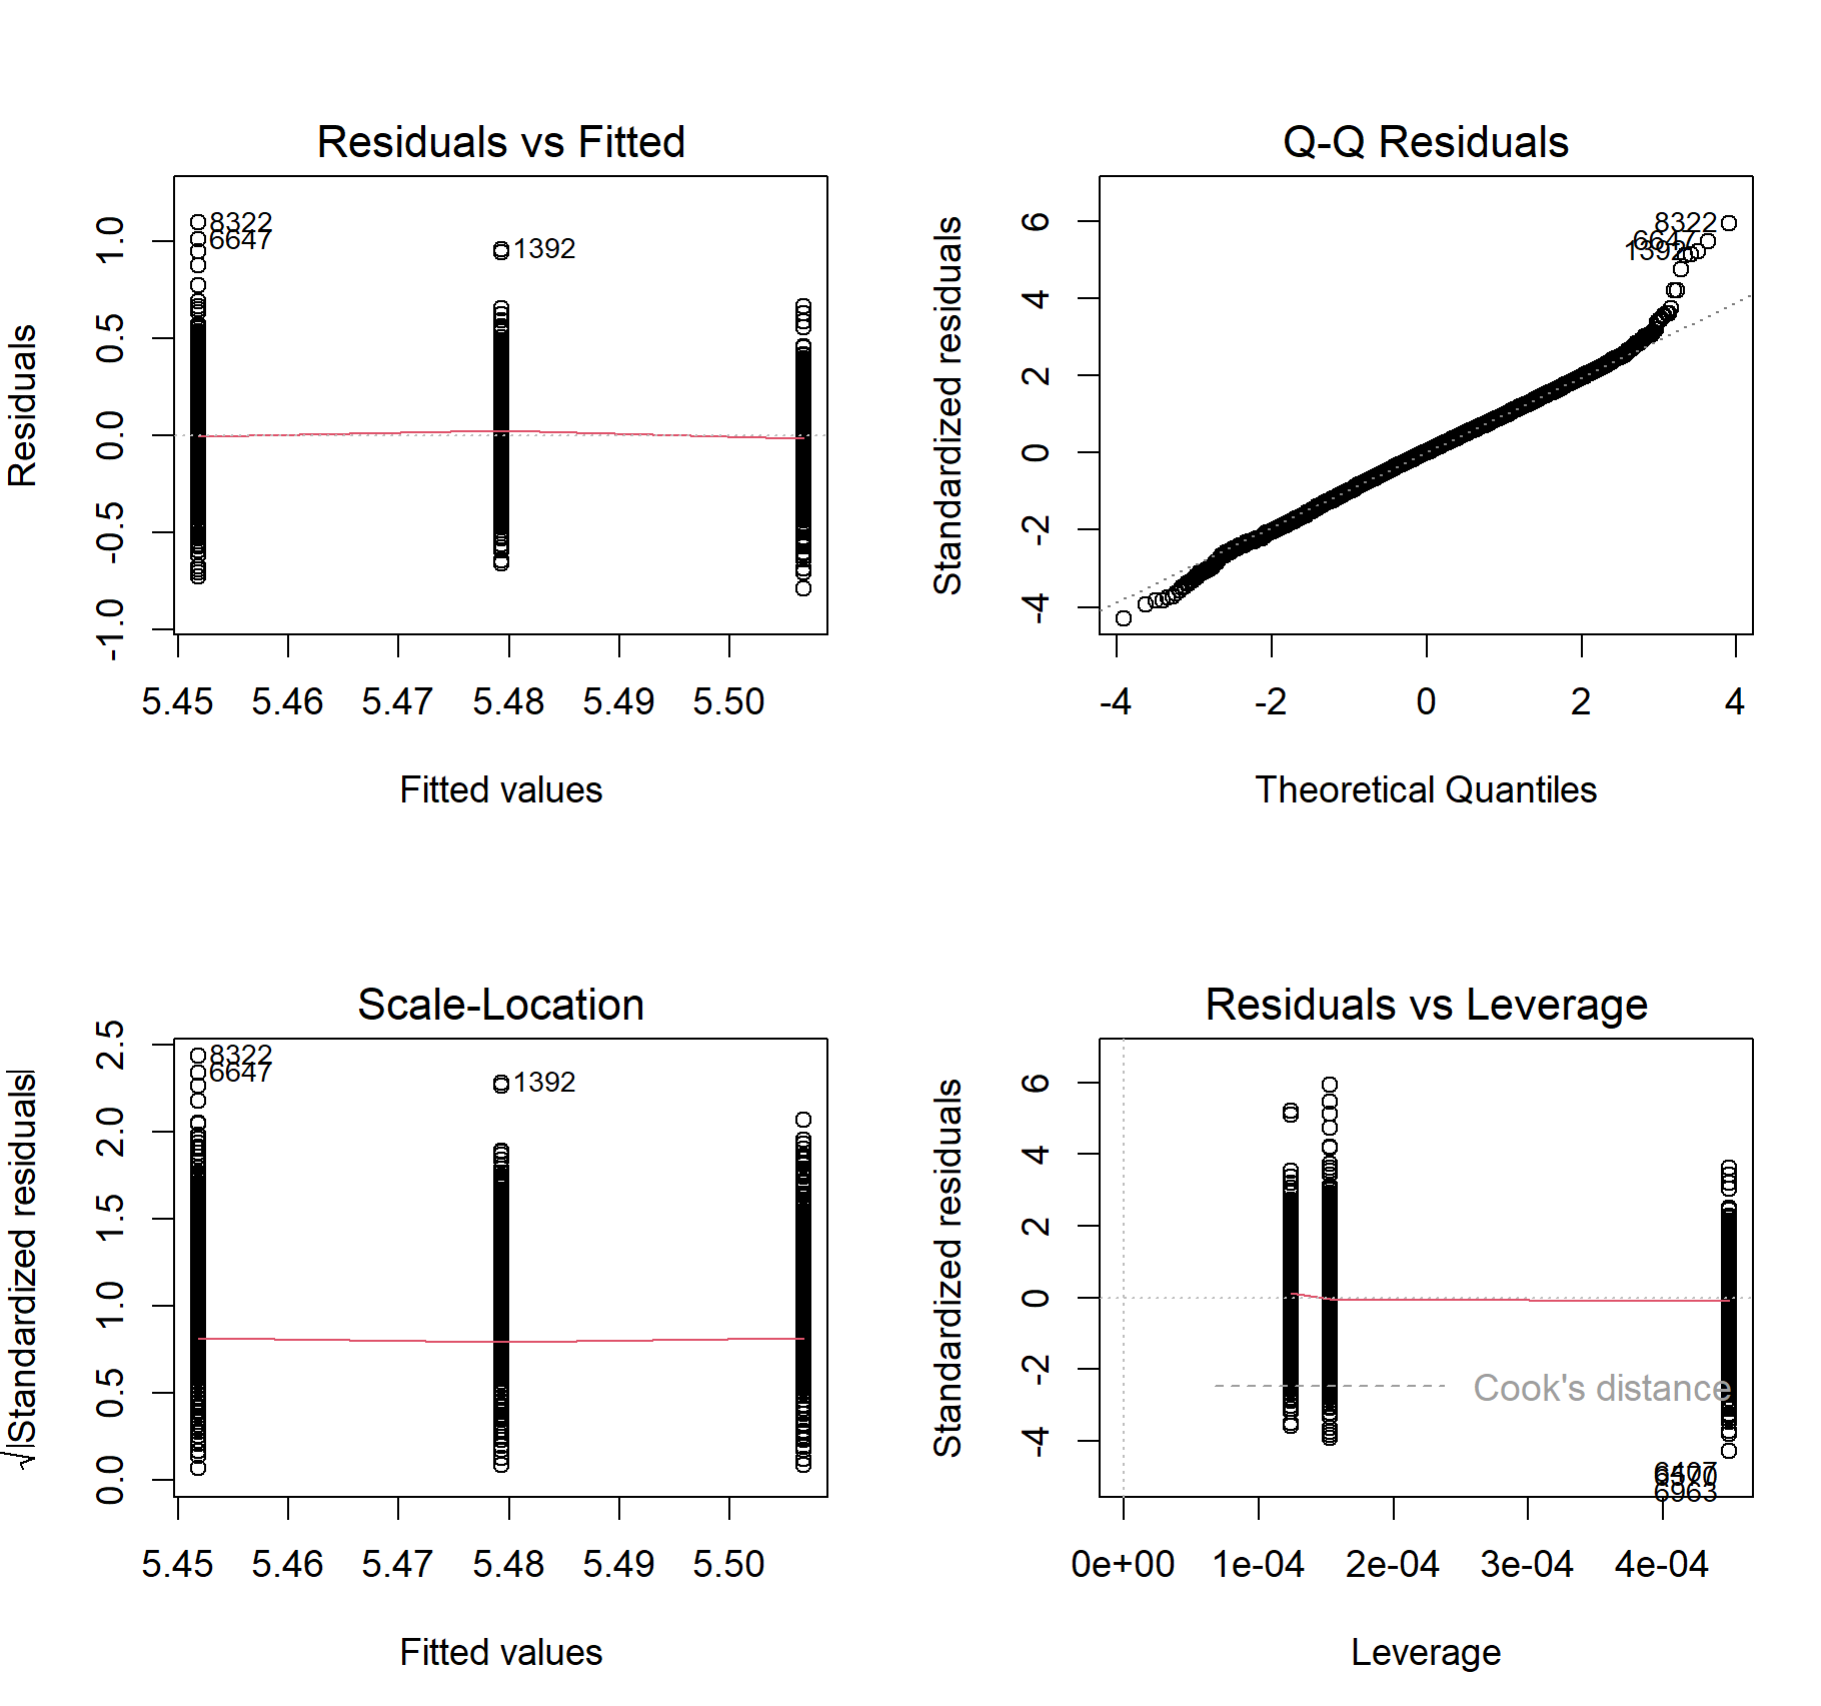
\includegraphics[width=0.8\textwidth]{figs/hw4_age_residuals.png}
\end{center}

\begin{itemize}
    \item normality：大部分点落在斜线上，说明基本服从正态，但发现右尾重尾。
    \item homogeneity：根据 Scale-Location 图，平方根标准化残差拟合线基本水平，虽然有少数离群值但是其整体分布均匀，没有出现明显的异方差情况。
\end{itemize}

综上，使用线性模型是合理的。

\subsubsection*{(iii)}

If the null hypothesis is rejected, perform a post-hoc test.

\textbf{Solution.}

\begin{verbatim}
$AGE_group
           diff         lwr          upr     p adj
2-1  0.05384320  0.04447619  0.063210213 0.0000000
3-1  0.03811704  0.02573994  0.050494134 0.0000000
3-2 -0.01572616 -0.02912186 -0.002330471 0.0163568
\end{verbatim}

如上说明各组之间均有显著关系，且1-2，1-3组间十分显著。

\subsection*{(c)}

Fit an \textbf{ANOVA} model of the outcome on \textbf{sex}.

\subsubsection*{(i)}

Test the null hypothesis of no sex effect. Visualize the data to check their relationship.

\textbf{Solution.}

\begin{center}
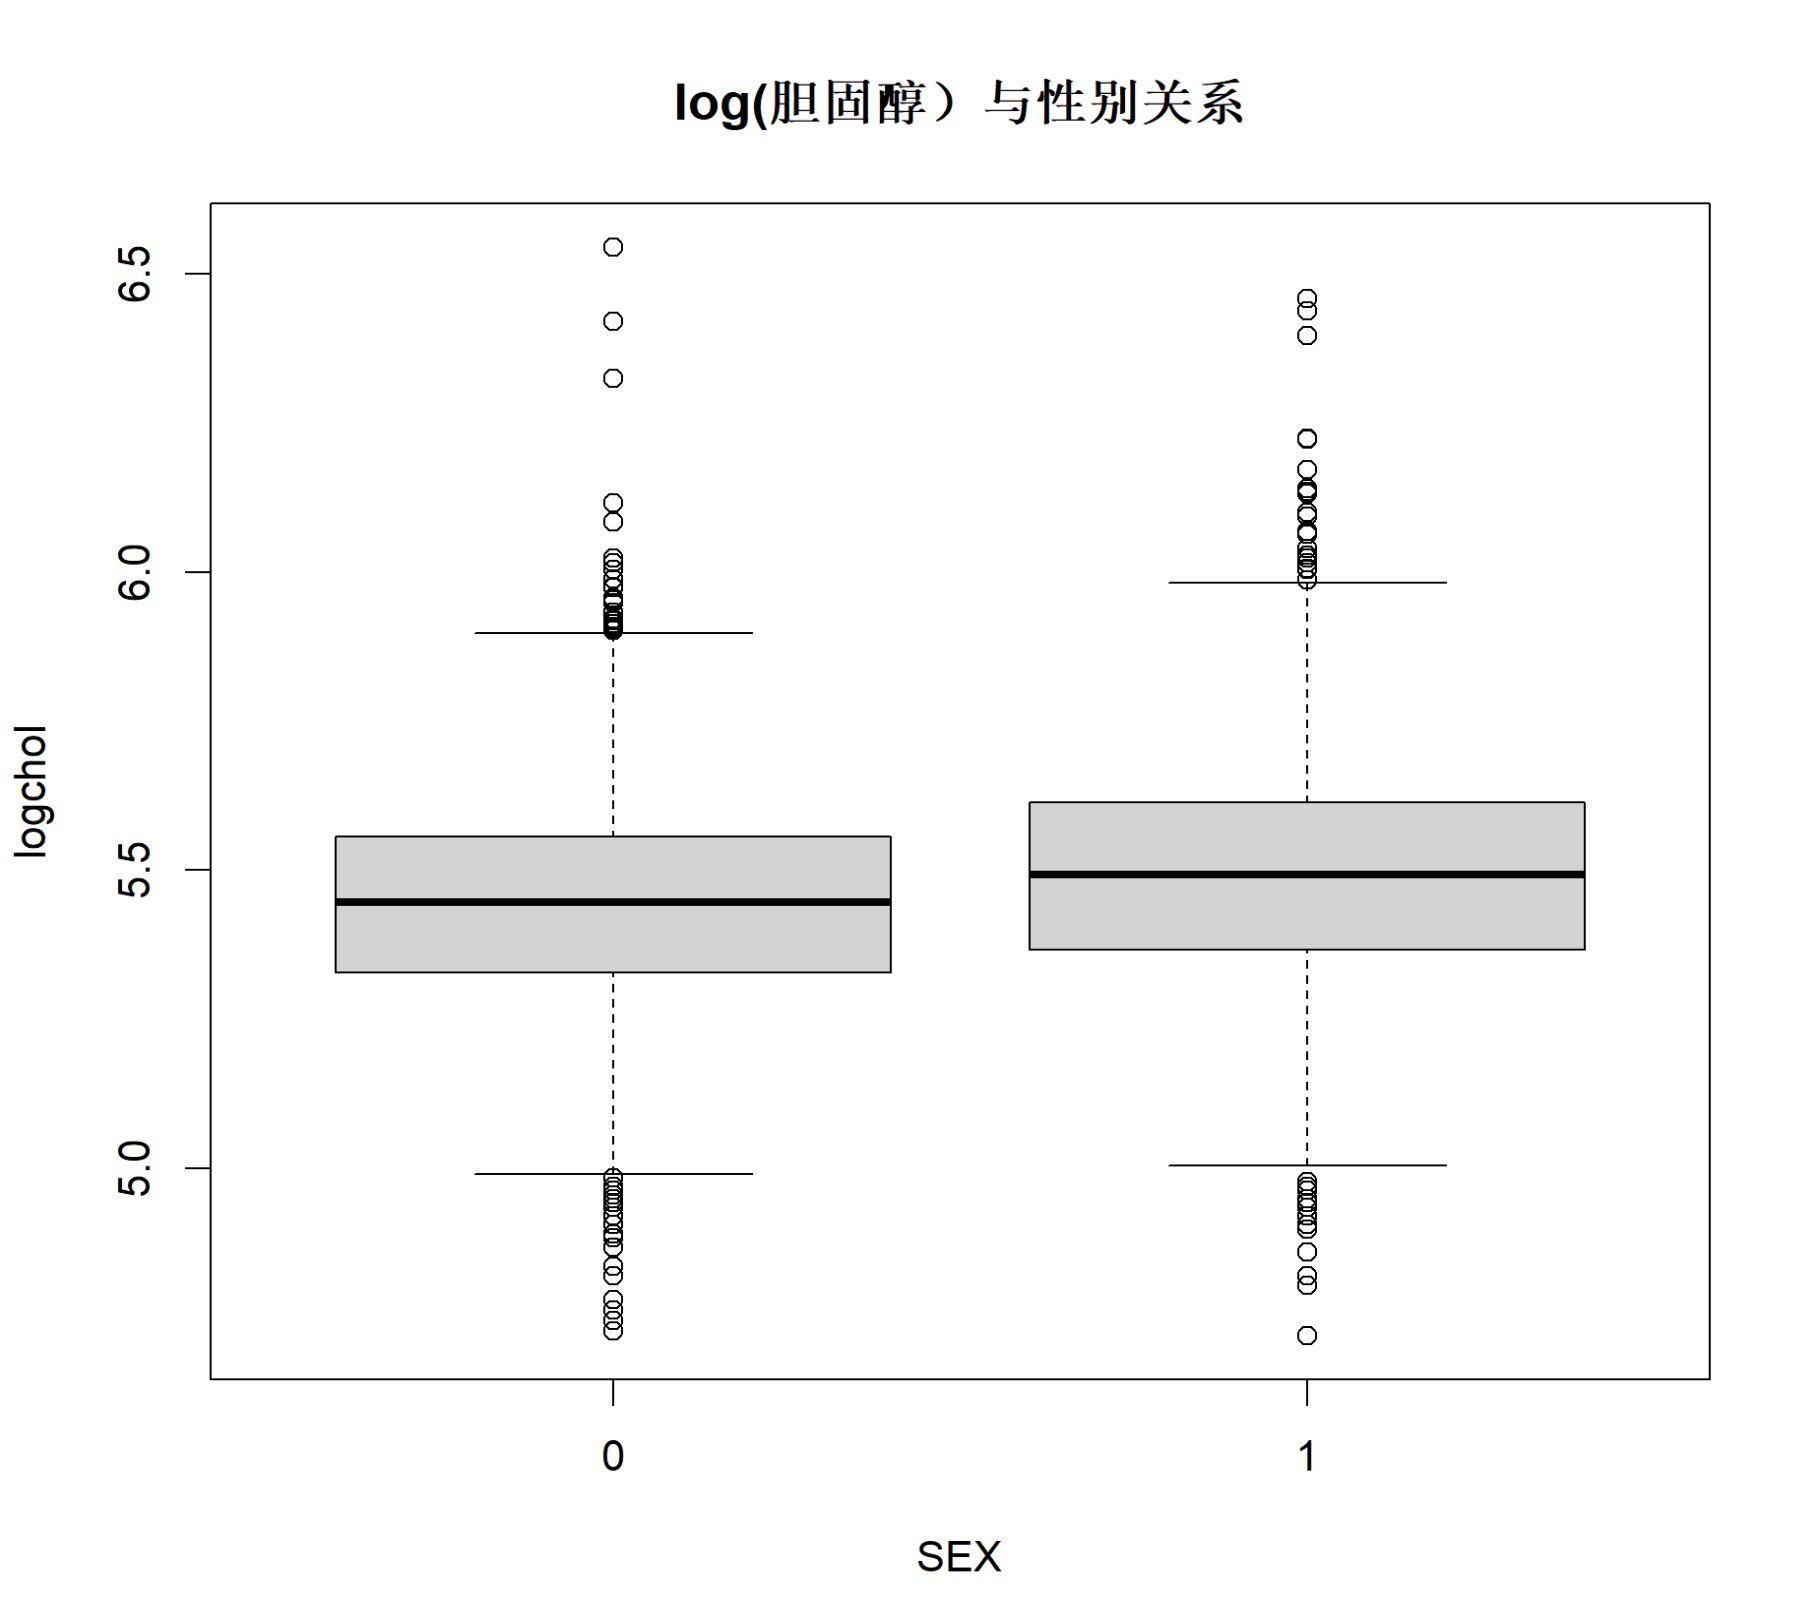
\includegraphics[width=0.7\textwidth]{figs/hw4_sex_boxplot.png}
\end{center}

$p\text{-value} < 2 \times 10^{-16}$，拒绝原假设。

\subsubsection*{(ii)}

Plot the residuals to assess the normality and homogeneity of errors.

\textbf{Solution.}

\begin{center}
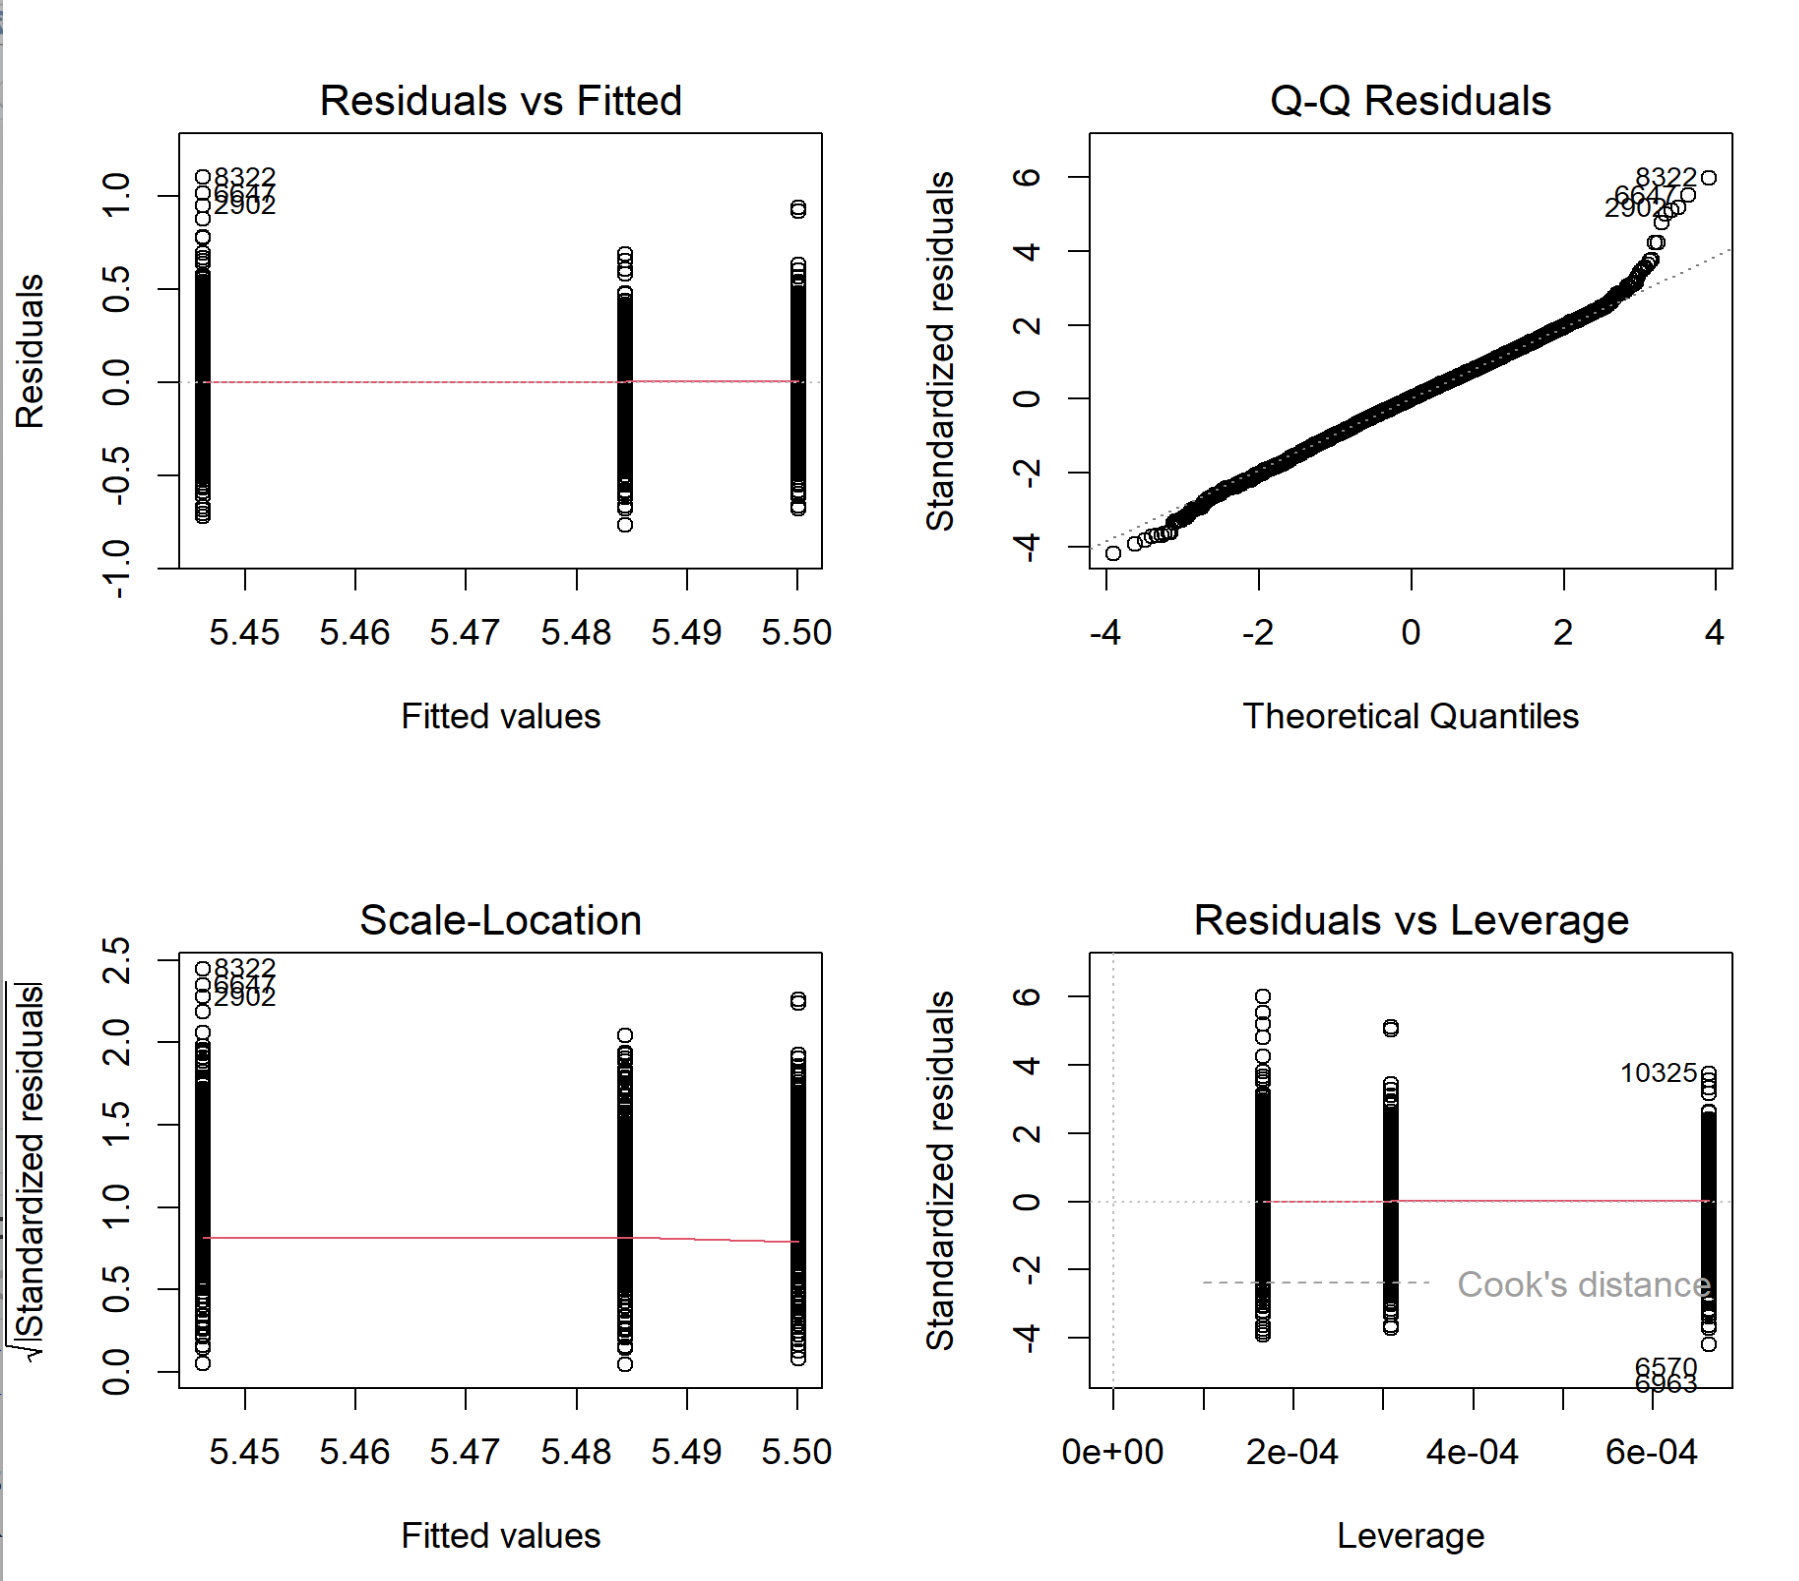
\includegraphics[width=0.8\textwidth]{figs/hw4_sex_residuals.png}
\end{center}

\begin{itemize}
    \item normality：大部分点落在斜线上，说明基本服从正态，但发现右尾重尾。
    \item homogeneity：根据 Scale-Location 图，平方根标准化残差拟合线基本水平，虽然有少数离群值但是其整体分布均匀，没有出现明显的异方差情况。
\end{itemize}

综上，使用线性模型是合理的。